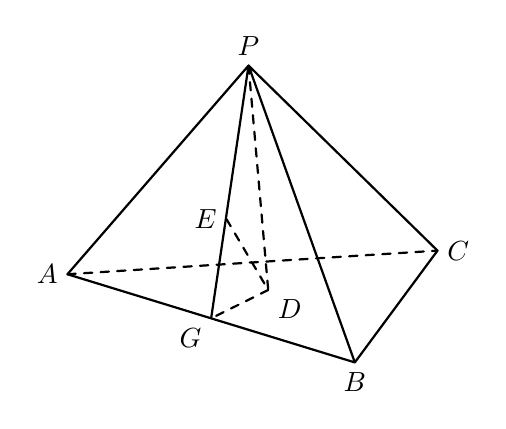
\begin{tikzpicture}[line cap=round,line join=round]
\coordinate (A) at (0,0);
\coordinate (B) at (3.65,-1.12);
\coordinate (C) at (4.7,0.3);
\coordinate (P) at (2.3,2.65);
\coordinate (G) at (1.825,-0.56);
\coordinate (E) at (2.02,0.70);
\coordinate (D) at (2.55,-0.20);

% 隐线与内部构造
\draw[thick,dashed] (A)--(C) (P)--(D) (E)--(D) (D)--(G);
% 棱与 PE 延长线 PG
\draw[thick] (A)--(B)--(C) (A)--(P) (B)--(P) (C)--(P) (P)--(G);

\node[left] at (A) {$A$};
\node[below] at (B) {$B$};
\node[right] at (C) {$C$};
\node[above] at (P) {$P$};
\node[left] at (E) {$E$};
\node[below right] at (D) {$D$};
\node[below left] at (G) {$G$};
\end{tikzpicture}
